\documentclass[a4paper,12pt]{article}
\usepackage[slovene]{babel}
\usepackage[utf8]{inputenc}
\usepackage[T1]{fontenc}
\usepackage{amsmath}
\usepackage{graphicx}
\usepackage{lmodern}
\usepackage{amsfonts}
\usepackage{amsthm}
\pagestyle{empty}

% Definicija okolij izrek, posledica
{\theoremstyle{plain}
\newtheorem{izrek}{Izrek}%[section]
\newtheorem{lema}[izrek]{Lema}
}
% Definicija okoli za definicije in vaje
{\theoremstyle{definition}
\newtheorem{definicija}[izrek]{Definicija}
\newtheorem{vaja}[izrek]{Vaja}
}


\usepackage{subfig}
\usepackage{graphicx}
\graphicspath{{./slike/}}


\title{Gregoryjeve krpe\\
\Large seminarska naloga}

\date{}
\author{Klara Kresnik in Meta Trdin\\
2. letnik\\
Fakulteta za matematiko in fiziko\\
}

%\address{Fakulteta za matematiko in fiziko}

\newcounter{definicija}
\newcommand{\tbf}{\textbf}

%\newenvironment{definicija}
%{
%	\refstepcounter{definicija}
%	\begin{flushleft}
%		\textbf{Definicija \arabic{definicija}:}
%}{
%	%\hfill $\square$ ta hfill sam nardi presledek pred definicijo
%	\end{flushleft} 
%}

%poišči kako se poravna besedilo
%naj bo prva stran cela samo naslov in zacni na drugi strani

\begin{document}
\maketitle
% še kera fakulteta
%predmet seminar
%drugi letnik
\pagebreak



\section{Uvod}
%presdtavitev problema
Za začetek najprej predstavimo problem. Krpe oziroma ploskve v prostoru želimo zlepiti tako, da bo vzdolž skupnega roba dosežena geometrijska zveznost reda 1. To bomo lahko dosegli lokalno. Zaradi lokalne $G^1$ zveznosti se Gregoryjeve krpe uporablja pri geometrijskem modeliranju in v računalniški grafiki. S predavanj vemo, da nam $G^1$ zveznost zagotavlja zveznost enotskih tangent, kar v našem primeru pomeni, da se morata tangentni ravnini ene in druge krpe ujemati.

Ko združujemo dve krpi, naletimo na problem. Reče se mu twist compatibility problem ali tudi vertex inconsistency problem in sicer ni nujno, da bodo mešani odvodi enaki.
Kot vemo se pri polinomski konstrukciji mešani odvodi ujemajo, v primeru Gregoryjevih krp pa niti ni treba, da se (glej sliko \ref{fig:mesani odvodi}). To je tudi ena izmed prednosti. Pokaže se pri računanju notranjih kontrolnih točk, kjer bo posamezna točka postala racionalna funkcija, zato bo ploskev sama po sebi racionalna.

\begin{figure}[h]
	\centering
	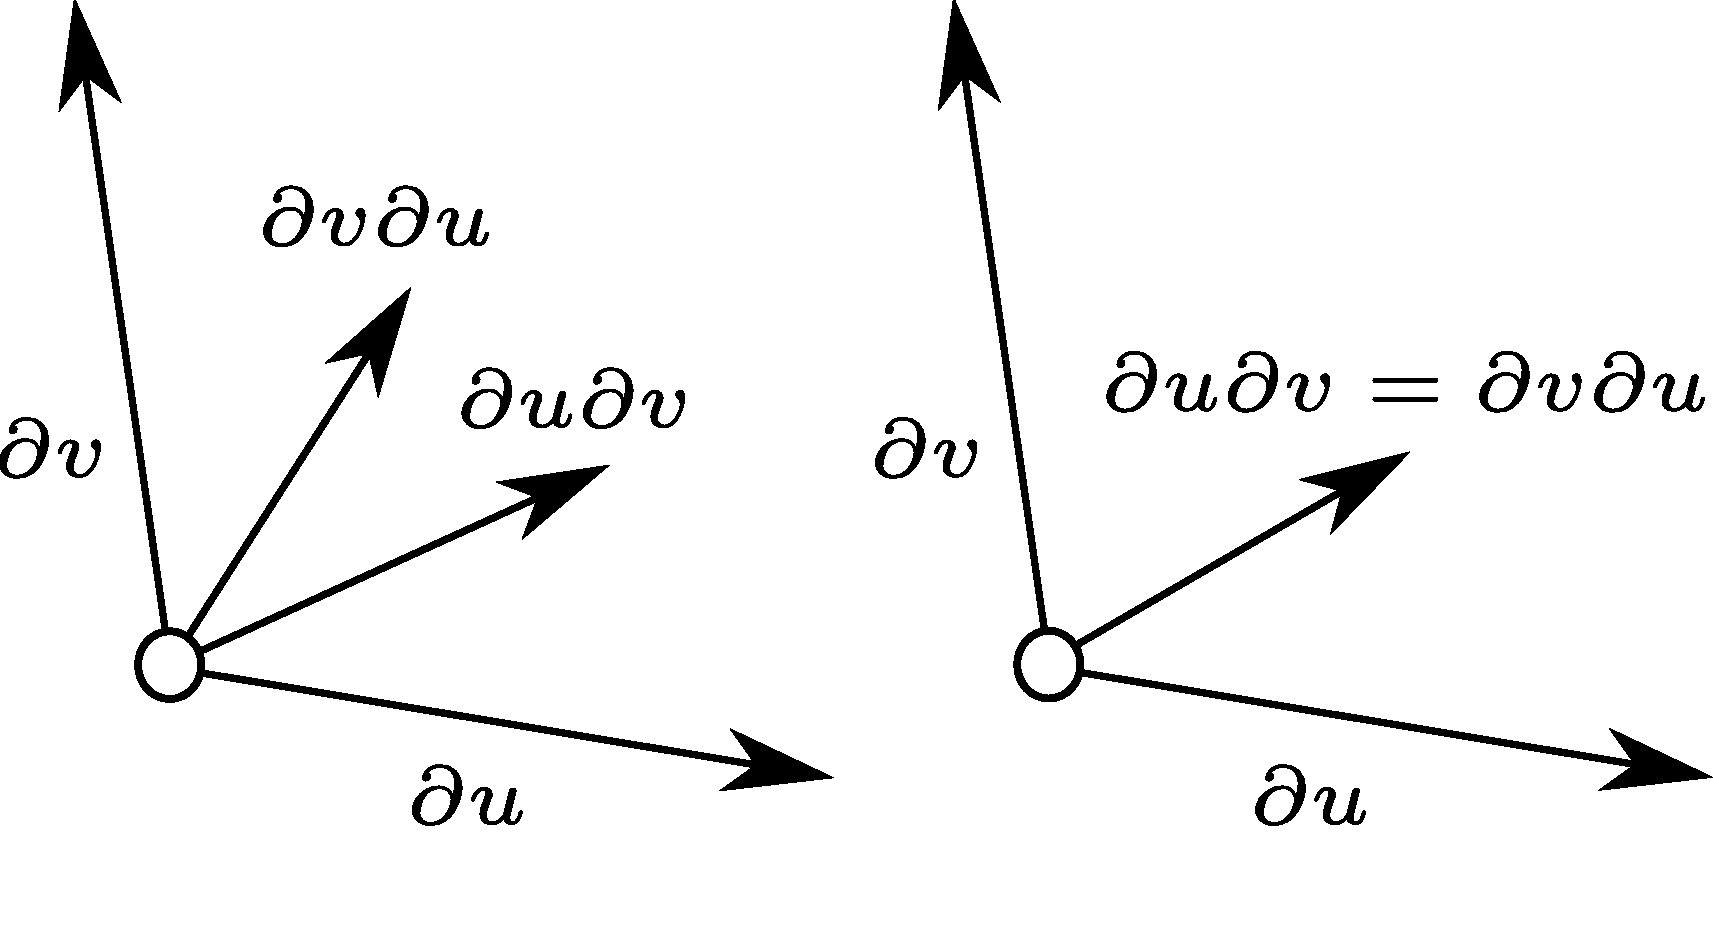
\includegraphics[width=7cm]{mesani_odvodi_ob.jpg}
	\caption{Levo: mešani odvodi v primeru Gregoryjeve krpe; Desno: mešani odvodi pri polinomski konstrukciji}
	\label{fig:mesani odvodi}
\end{figure}

Podane bomo imeli robne krivulje, ki bodo kar bezierjeve krivulje stopnje $3$. Računali bomo notranje kontrolne točke. Pri tem bomo potrebovali tudi podatke s tangentne ravnine na robu, da bomo lahko zagotovili $G^1$ zveznost. To nas pripelje do metode Chiyokura in Kimura. 


\section{metoda Chiyokura in Kimura}
\begin{itemize}
	\item metoda združi dve Bezierjevi krpi tako, da zagotavlja geometrijsko zv reda 1
	\item upošteva le robne krivulje in	
\end{itemize}
 


\section{Gregorijeve krpe}


\begin{itemize}
	\item Z gregoryjevimi krpami posplošimo gregorijeve ideje za tenzorski produkt bezierjevih krp(mogoče se tuki kej dodaš)
	\item skonstruirati želimo ploskev, ki bo imela geometrjsko zv reda 1 ko jo bomo zlepili še z drugimi ploskvami
	\item podane imamo le robne krivulje
	\item povej tudi da jih lahko delamo nad večkotniki ampak da sva se medve ukvarjali le s trikotnimi in 4kotnimi.
\end{itemize}

Poglejmo si kontrukciji štirikotne in trikotne Gregoryjeve krpe.

\subsection{Kvadratne Gregoryjeve krpe}

\begin{itemize}
	\item  Domena $u,v \in [0,1] \times [0,1]$
	\item Imamo štiri kubične bezierjeve krivulje, vsaka bredstavlja rob gregorijeve krpe.
	\item na vsakem robu nato uporabimo metodo Chiyokura in Kimura: na vsakem robu dobimo 2 točki, torej skupaj $8$. tako zagotovimo G1 zveznost.
	\item tukaj nastopi twist compatibility problem-točke se ne ujemajo
	\item zato bomo uporabili racionalne funkcije (pomagali si bomo z rac funkcijami)
	\item za vsako vozliošče ena funkcija torej 4 funkcije
	\item formule
	\item te funkcije so definirane tako zato, da dobimo če vstavimo $\tbf{b}_{11}(0,v) = \tbf{b}_{11,u_0}$ itd
\end{itemize}

\begin{align*}
\textbf{b}_{11(u,v)} &=  \frac{v \textbf{b}_{11,u_0}+u\tbf{b}_{11,v_0}}{u +v} \\
\tbf{b}_{21}(u,v) &= \frac{(1-v) \tbf{b}_{21,u_0}+u\tbf{b}_{21,v_1}}{(1-v)+u} \\
\tbf{b}_{12}(u,v) &= \frac{v \tbf{b}_{12,u_1}+(1-u)\tbf{b}_{12,v_0}}{v+(1-u)} \\
\tbf{b}_{22}(u,v) &= \frac{(1-v) \tbf{b}_{22,u_1}+(1-u)\tbf{b}_{22,v_1}}{(1-u)+(1-v)} 
\end{align*}	

\subsection{Trikotne Gregoryjeve krpe}
\begin{itemize}
	\item trikotna domena
	\item tokrat imamo 3 kubicne bezierjeve krivulje na robu
	\item spet uporabimo metodo in dobimo 6 točk (3 pare točk)
	\item na posameznem paru uporabim racionalno funkcijo da dobimo 3 notranje točke kvadratične bezierjeve krpe. kubična bezierjeva krpa ima le eno kontrolno točko ki ni robna, kvadratna pa ima 3 kar nam v tem primeru bolj ustreza. Zato moramo še robnim krivuljam zvišati stopnjo.
\end{itemize}


\begin{align*}
\tbf{b}_{211} &= \frac{(1-w)v \tbf{b}_{211,uv}+(1-v)w\tbf{b}_{211,v_1}}{(1-w)v+(1-v)w} \\
\tbf{b}_{121} &= \frac{(1-w)u \tbf{b}_{121,uv}+(1-u)v\tbf{b}_{121,vw}}{(1-w)u+(1-u)w} \\
\tbf{b}_{112} &= \frac{(1-u)v \tbf{b}_{112,vw}+(1-v)u\tbf{b}_{112,uw}}{(1-u)v+(1-v)u} 
\end{align*}

\section{Zaključek}



\begin{thebibliography}{99}
	% to so primeri,kasneje jih pobriši
	
	\bibitem{osnovni-clanek}
	R.~Akhtar, T.~Jackson-Henderson, R.~Karpman, M.~Boggess, I.~Jimenez, A.~Kinzel, D.~Pritikin, \emph{On the unitary Cayley graph of a finite ring}, Electron.\ J. Combin.\ \textbf{16} (2009), no. 1,\ Research Paper 117,\ 13 pp.
	
	\bibitem{koncen_produkt}
	M.~F.~Atiyah, I.~G.~MacDonald. \emph{Introduction to Commutative Algebra}, Addison-Wesley-Longman, 1969
	
	%I.~Priimek, \emph{Naslov knjige}, morebitni naslov zbirke  \textbf{zaporedna številka}, založba, kraj, leto izdaje.
	
	\bibitem{tenzorji}
	K.~Schäcke, \emph{On the Kronecker product}, 2013
	
	\bibitem{vir_10}
	M.~E.~Watkins, \emph{Connectivity of transitive graphs}, J.~Combin.\ Theory \textbf{8} (1970), 23-29.
	
	\bibitem{vir_11}
	D.~B.~West. \emph{Graph Theory}, Second Edition.\ Prentice-Hall, (2000).
	
\end{thebibliography}














\end{document}